\chapter{Évolution moléculaire et phylogénomique}\label{ch:b3:molecular-evolution}

En 1968 Motoo Kimura fit un calcul qui troubla une discipline. En
comparant les hémoglobines, les cytochromes et d'autres protéines de
mammifères dont les ancêtres communs étaient datés par les fossiles, il
trouva que les acides aminés avaient été remplacés au rythme d'environ
une substitution par site et par milliard d'années --- ce qui, sur un
génome de mammifère et par génération, revenait à une nouvelle
substitution fixée dans la population tous les deux ans environ. Haldane
avait montré dix ans plus tôt que la sélection naturelle ne peut fixer
qu'environ une substitution toutes les trois cents générations avant que
le coût en descendants perdus devienne impayable. L'arithmétique ne
laissait qu'une issue~: la plupart des changements qui s'accumulent dans
l'ADN ne sont pas mus par la sélection, mais sont neutres, fixés par
hasard dans des populations finies, à un rythme qui --- comme le montre
le premier théorème de ce chapitre --- est simplement le taux de
mutation. La \omterm{thm:b3:molecular-evolution:neutral}{théorie neutraliste} est devenue l'hypothèse nulle de
l'évolution moléculaire, la référence face à laquelle on détecte la
sélection~; l'\omterm{prop:b3:molecular-evolution:clock}{horloge moléculaire} est devenue un moyen de dater ce que
les fossiles ne pouvaient pas~; et les génomes séquencés depuis ont
donné les outils pour voir, gène par gène, où la sélection a agi,
comment des gènes neufs naissent d'anciens, et pourquoi l'arbre d'un
gène n'est pas toujours celui de son espèce.

\section{Dérive, mutation et taux neutre}

\begin{theorem}[Le taux de substitution neutre]\label{thm:b3:molecular-evolution:neutral}
\index{théorie neutraliste}\index{taux de substitution}\index{probabilité de fixation}\index{dérive génétique}
Dans une population diploïde de $N$ individus, une nouvelle mutation
sans effet sur la valeur sélective a une probabilité $1/2N$ de finir par
remplacer tous les autres allèles (la \emph{fixation}) et $1 - 1/2N$
d'être perdue. Si chacune des $2N$ copies du gène mute au taux $\mu$ par
génération, $2N\mu$ nouvelles mutations neutres apparaissent par
génération et, à long terme, le rythme d'accumulation des substitutions
vaut
\[
k = 2N\mu\times\frac{1}{2N} = \mu :
\]
le \emph{\omterm{thm:b3:molecular-evolution:neutral}{taux de substitution}} neutre égale le taux de mutation,
indépendamment de la taille de la population. Une mutation destinée à se
fixer met en moyenne $4N$ générations à le faire, de sorte que les
grandes populations tiennent plus de variation en transit mais ne la
fixent pas plus vite. Pour une mutation d'avantage sélectif $s$, la
formule de Kimura donne la \omterm{thm:b3:molecular-evolution:neutral}{probabilité de fixation}
\[
P(s) = \frac{1 - \mathrm{e}^{-2s}}{1 - \mathrm{e}^{-4Ns}} \approx 2s
\quad (4Ns \gg 1),
\]
de sorte qu'un avantage de \qty{1}{\%} se fixe avec une probabilité
d'environ \qty{2}{\%} --- quarante fois la chance d'une mutation neutre
dans une population de deux mille individus, mais tout de même perdue
quarante-neuf fois sur cinquante~; et un désavantage $s < 0$ avec
$4N|s| \gg 1$ ne se fixe pour ainsi dire jamais, tandis qu'un
désavantage avec $4N|s| \ll 1$ se comporte comme neutre~: la sélection
ne voit que ce que la dérive ne noie pas, et la frontière est $|s| \sim
1/4N$ --- l'\emph{effectivement neutre}.
\end{theorem}
\begin{proof}
La neutralité~: une copie présente aujourd'hui sera l'ancêtre de toute
la population dans un lointain avenir, et par symétrie chacune des $2N$
copies a la même chance de l'être~; le nouveau mutant est une copie,
d'où $1/2N$. Le taux~: substitutions par génération $=$ (mutations
apparaissant par génération) $\times$ (probabilité que chacune se fixe)
$= 2N\mu/2N$. La formule de Kimura découle de l'approximation de
diffusion pour la variation de fréquence allélique sous la dérive et la
sélection, admise ici~; ses limites se vérifient directement~: quand
$s \to 0$, $(2s)/(4Ns) = 1/2N$, la valeur neutre~; pour $4Ns \gg 1$ le
dénominateur vaut $1$ et le numérateur $\approx 2s$. Le temps de
fixation~: la fréquence d'un allèle neutre suit une marche au hasard de
variance $p(1-p)/2N$ par génération, et le temps attendu pour atteindre
$1$ depuis $1/2N$, sachant qu'on y parvient, vaut $4N$ générations
(Kimura et Ohta, 1969), admis.
\end{proof}

\begin{omfigure}
\begin{tikzpicture}
\begin{semilogyaxis}[
  width=0.62\linewidth, height=5.6cm,
  axis x line=bottom, axis y line=left,
  xmin=-4, xmax=8, ymin=0.00002, ymax=0.2,
  xlabel={$4Ns$ (coefficient de sélection mis à l'échelle)}, ylabel={probabilité de fixation},
  xlabel style={font=\small, at={(axis description cs:0.5,-0.12)}, anchor=north}, ylabel style={font=\small},
  tick label style={font=\small}, xtick={-4,-2,0,2,4,6,8}, ytick={0.0001,0.001,0.01,0.1}, yticklabels={$10^{-4}$,$10^{-3}$,$10^{-2}$,$10^{-1}$},
  clip=false,
]
\addplot[very thick, omDef, domain=-4:-0.05, samples=60] {(x/2000)/(1-exp(-x))};
\addplot[very thick, omDef, domain=0.05:8, samples=80] {(x/2000)/(1-exp(-x))};
\draw[dashed, gray] (axis cs:-4,0.0005) -- (axis cs:8,0.0005); \node[font=\scriptsize, gray, anchor=north west] at (axis cs:-3.9,0.00048) {neutre, $1/2N$};
\addplot[thick, omThm, dashed, domain=1:8, samples=2] {2*x/(4*1000)};
\node[font=\scriptsize, omThm, anchor=north west] at (axis cs:5,0.0012) {asymptote $2s$};
\node[font=\scriptsize, omDef, anchor=south east, align=right] at (axis cs:-0.2,0.02) {effectivement neutre\\quand $|4Ns| \lesssim 1$};
\node[font=\scriptsize, omDef, anchor=south west] at (axis cs:-3.9,0.0008) {délétère~: presque jamais fixée};
\end{semilogyaxis}
\end{tikzpicture}

{\small La \omterm{thm:b3:molecular-evolution:neutral}{probabilité de fixation} de Kimura en fonction du coefficient
de sélection mis à l'échelle, pour $N = 1000$. Près de zéro la courbe
passe par la valeur neutre~; à droite elle monte vers $2s$~; à gauche
elle tombe d'une falaise. La sélection n'agit que sur ce que la dérive
ne peut cacher.}
\end{omfigure}

\begin{proof}[Faits expérimentaux]
Kimura (1968) puis King et Jukes (1969) ont tiré l'argument des taux~:
le rythme observé de substitution des acides aminés dans les protéines
de mammifères impliquait plus de substitutions par génération que ne
l'autorisait le coût de la sélection de Haldane, de sorte que la plupart
devaient être neutres. Les prédictions de la théorie ont ensuite tenu~:
les taux sont les plus élevés là où la fonction contraint le moins ---
sites synonymes, introns, \omterm{def:b3:molecular-evolution:duplication}{pseudogènes}, troisième position du codon ---
et les plus bas dans les \omterm{def:b3:chromatin-epigenetics:nucleosome}{histones} et l'ubiquitine, qui changent d'un
résidu en cent millions d'années~; le niveau de variation à l'intérieur
d'une espèce suit la mutation et la taille de population~; et le rythme
de substitution par an est à peu près constant entre lignées de tailles
de population très différentes, comme l'exige la formule $k = \mu$ et
comme une explication sélectionniste ne le fait pas. La controverse qui
a suivi ne l'a pas renversée~: elle a fixé le taux neutre comme
l'hypothèse nulle face à laquelle on mesure la sélection.
\end{proof}

\begin{omfigure}
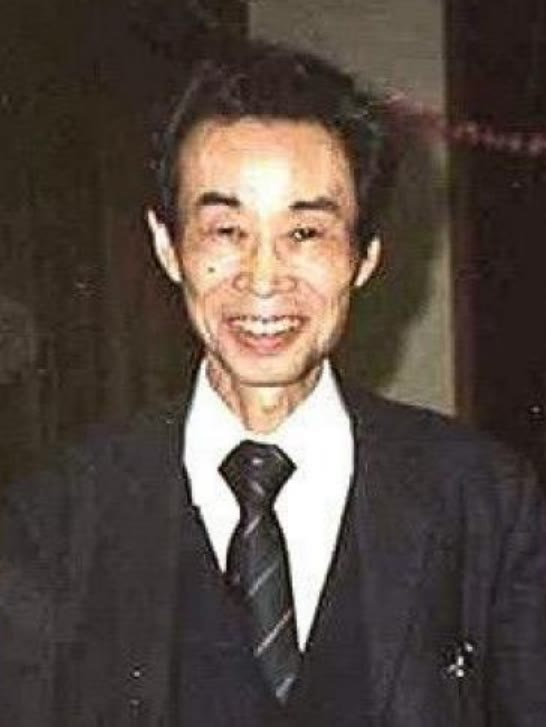
\includegraphics[width=0.34\linewidth]{images/book5/kimura.jpg}\hspace{0.05\linewidth}
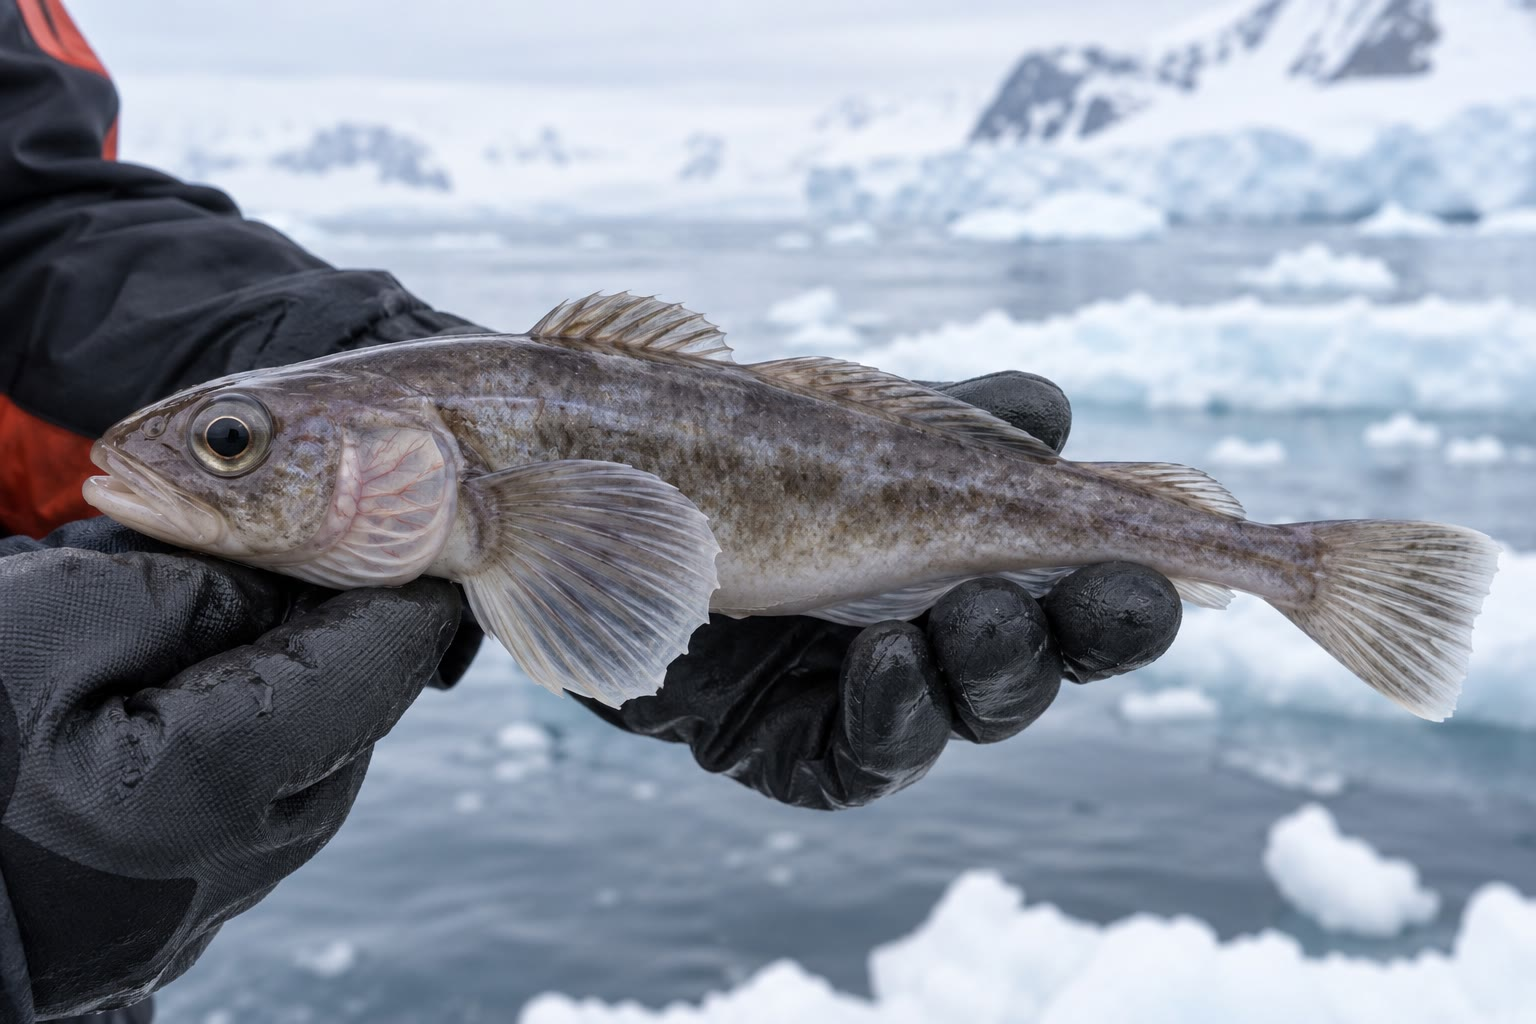
\includegraphics[width=0.5\linewidth]{images/book5/ai/b5-25-icefish.jpg}

{\small À gauche~: Motoo Kimura (1924--1994), qui a montré que
l'essentiel du changement moléculaire est fixé par hasard et au taux de
mutation (photographie, 1986, CC BY 4.0). À droite~: un poisson des
glaces de l'Antarctique, dont le sang est empêché de geler par une
glycoprotéine antigel assemblée, il y a une dizaine de millions
d'années, à partir d'un gène d'enzyme digestive dupliqué et d'une série
de répétitions.}
\end{omfigure}

\section{L'horloge moléculaire}

\begin{proposition}[L'horloge et ses irrégularités]\label{prop:b3:molecular-evolution:clock}
\index{horloge moléculaire}\index{calibration}\index{hétérogénéité des taux}\index{horloge relâchée}\index{effet du temps de génération}
Si les substitutions s'accumulent à un taux constant $k$ par site et par
an dans deux lignées séparées depuis $T$ années, la fraction de sites où
elles diffèrent vaut, pour de petites valeurs, $d \approx 2kT$~: la
divergence de deux séquences est une \emph{\omterm{prop:b3:molecular-evolution:clock}{horloge moléculaire}}
(Zuckerkandl et Pauling, 1965), qu'on peut \emph{calibrer} par une
séparation datée par un fossile puis lire pour des séparations sans
fossile. L'horloge est stochastique --- un processus de Poisson, de
sorte que $d$ a une variance à peu près égale à sa moyenne sur un nombre
fixé de sites --- et elle est irrégulière de trois façons connues.
Chaque protéine a son propre taux, fixé par la fraction de ses sites que
la fonction laisse changer~: fibrinopeptides à \num{8}, hémoglobine
\num{1}, cytochrome~$c$ \num{0.3}, \omterm{def:b3:chromatin-epigenetics:nucleosome}{histone}~H4 \num{0.01} substitutions
par site et par milliard d'années. Les taux diffèrent entre lignées~:
puisque le taux neutre est $\mu$ par génération, les animaux à
générations courtes (rongeurs) accumulent plus de changement par an que
ceux à générations longues (primates, baleines) --- l'\emph{\omterm{prop:b3:molecular-evolution:clock}{effet du
temps de génération}}, en partie compensé parce que les taux de mutation
par génération montent avec la durée des générations. Et $d$ sature~:
une fois que beaucoup de sites ont changé, les changements suivants
frappent des sites déjà changés, de sorte qu'il faut corriger la
différence brute pour les coups multiples, comme le font les distances
du chapitre sur l'\omterm{def:b3:bioinformatics:alignment}{alignement}. Les \emph{\omterm{prop:b3:molecular-evolution:clock}{horloges relâchées}} modernes
laissent le taux varier d'une branche à l'autre dans un modèle
statistique et sont calibrées par de nombreux fossiles à la fois~; elles
datent la séparation de l'humain et du chimpanzé à six ou sept millions
d'années, celle des ordres de mammifères placentaires près de la fin du
Crétacé, et celle des animaux et des champignons au Précambrien, avec
des incertitudes de dix à vingt pour cent qui viennent surtout des
fossiles.
\end{proposition}
\begin{proof}
Chaque lignée accumule $kT$ substitutions par site, de sorte que la
différence entre elles vaut $2kT$ là où les sites n'ont pas été frappés
deux fois~; une paire datée par un fossile donne $k = d/2T$. La variance
de Poisson et les taux par protéine sont ceux de Zuckerkandl et Pauling,
de Dickerson (1971) et des ajustements de Kimura à des jeux de protéines
de vertébrés~; la correction de saturation est la formule de
Jukes--Cantor du chapitre sur l'\omterm{def:b3:bioinformatics:alignment}{alignement}, $d_{\text{vrai}} =
-\tfrac{3}{4}\ln(1 - \tfrac{4}{3}p)$. La variation des taux entre
lignées a été montrée par les tests de taux relatifs~: avec un groupe
externe $O$ et deux espèces $A$, $B$, la différence $d_{AO} - d_{BO}$
devrait être nulle sous une horloge stricte, et ne l'est pas pour les
rongeurs face aux primates.
\end{proof}

\begin{omfigure}
\begin{tikzpicture}
\begin{axis}[
  width=0.68\linewidth, height=5.8cm,
  axis x line=bottom, axis y line=left,
  xmin=0, xmax=600, ymin=0, ymax=110,
  xlabel={temps depuis la divergence (millions d'années)}, ylabel={substitutions pour 100 sites (corrigées)},
  xlabel style={font=\small, at={(axis description cs:0.5,-0.12)}, anchor=north}, ylabel style={font=\small},
  tick label style={font=\small}, xtick={0,100,200,300,400,500,600}, ytick={0,20,40,60,80,100},
  clip=false,
]
\addplot[very thick, omThm, domain=0:130, samples=2] {2*0.4*x};
\addplot[very thick, omDef, domain=0:600, samples=2] {2*0.09*x};
\addplot[very thick, omMeth!70!black, domain=0:600, samples=2] {2*0.03*x};
\addplot[very thick, omProp!80!black, domain=0:600, samples=2] {2*0.001*x};
\addplot[only marks, mark=*, mark size=1.8pt, omDef] coordinates {(80,13) (100,20) (300,52) (400,75) (450,80)};
\addplot[only marks, mark=*, mark size=1.8pt, omMeth!70!black] coordinates {(80,4) (300,17) (450,29) (550,33)};
\addplot[only marks, mark=*, mark size=1.8pt, omThm] coordinates {(30,22) (80,68) (100,80)};
\node[font=\scriptsize, omThm, anchor=west] at (axis cs:132,104) {fibrinopeptides};
\node[font=\scriptsize, omDef, anchor=south east] at (axis cs:600,108) {hémoglobine};
\node[font=\scriptsize, omMeth!70!black, anchor=north west] at (axis cs:530,35) {cytochrome $c$};
\node[font=\scriptsize, omProp!80!black, anchor=south east] at (axis cs:600,1.5) {histone H4};
\end{axis}
\end{tikzpicture}

{\small L'\omterm{prop:b3:molecular-evolution:clock}{horloge moléculaire}, protéine par protéine. Chacune tourne à
son propre rythme, fixé par la part de la molécule que la fonction
laisse libre de changer~: un fibrinopeptide, coupé et jeté quand le sang
coagule, change des centaines de fois plus vite que l'\omterm{def:b3:chromatin-epigenetics:nucleosome}{histone} qui
empaquette l'ADN.}
\end{omfigure}

\section{Lire la sélection dans les séquences}

\begin{definition}[Le rapport dN/dS]\label{def:b3:molecular-evolution:dnds}
\index{substitution synonyme}\index{substitution non synonyme}\index{rapport dN/dS}\index{sélection purificatrice}\index{sélection positive}
Dans un gène codant, une substitution est \emph{synonyme} si elle laisse
l'acide aminé inchangé et \emph{non synonyme} si elle le change. Comme
le code génétique laisse la plupart des troisièmes positions et
certaines premières positions changer silencieusement, environ un quart
des mutations possibles d'un gène typique sont synonymes. Soit $d_{S}$
le nombre de substitutions synonymes par site synonyme et $d_{N}$ les
substitutions non synonymes par site non synonyme, chacun corrigé pour
les coups multiples. Les changements synonymes sont proches de la
neutralité, de sorte que $d_{S}$ estime $2\mu T$ --- l'horloge~; et le
rapport
\[
\omega = \frac{d_{N}}{d_{S}}
\]
mesure ce que la sélection a fait à la protéine~: $\omega = 1$ si les
changements d'acide aminé sont aussi libres que les silencieux (aucune
contrainte, comme dans un \omterm{def:b3:molecular-evolution:duplication}{pseudogène})~; $\omega < 1$ sous
\emph{sélection purificatrice}, la plupart des changements étant retirés
--- le gène typique a $\omega \approx 0.1$ à $0.2$, les \omterm{def:b3:chromatin-epigenetics:nucleosome}{histones} $0.001$~;
$\omega > 1$ sous \emph{sélection positive}, les changements d'acide
aminé étant favorisés plus vite que la dérive seule ne l'autorise --- le
sillon de liaison à l'\omterm{def:b3:adaptive-immunity:lymphocytes}{antigène} des molécules du CMH, les protéines de
surface des \omterm{def:b3:virology:virus}{virus} en course aux armements avec les \omterm{def:b3:adaptive-immunity:antibody}{anticorps}, les
protéines du spermatozoïde et de l'ovule lors de la fécondation, et le
lysozyme des ruminants, recruté pour digérer les bactéries dans
l'estomac. Calculé le long d'une branche d'un arbre ou site par site,
$\omega$ cartographie où et quand une protéine a été changée par la
sélection plutôt que par le hasard.
\end{definition}

\begin{omfigure}
\begin{tikzpicture}[every node/.style={font=\scriptsize}, >=stealth]
  \begin{axis}[
    width=0.52\linewidth, height=5.2cm,
    xbar, bar width=7pt, y=0.45cm,
    axis x line=bottom, axis y line=left,
    xmin=0.0005, xmax=5, xmode=log,
    xlabel={$\omega = d_{N}/d_{S}$},
    xlabel style={font=\small, at={(axis description cs:0.5,-0.12)}, anchor=north},
    symbolic y coords={histone H4, actin, insulin, typical gene, cytochrome $c$, pseudogene, ruminant lysozyme, MHC groove, HIV envelope},
    ytick=data, yticklabels={histone H4, actine, insuline, gène typique, cytochrome \textit{c}, pseudogène, lysozyme de ruminant, sillon du CMH, enveloppe du VIH}, tick label style={font=\scriptsize},
    xtick={0.001,0.01,0.1,1}, xticklabels={0.001,0.01,0.1,1},
    clip=false,
  ]
  \addplot[fill=omDef!50, draw=omDef] coordinates {(0.002,histone H4) (0.01,actin) (0.09,insulin) (0.15,typical gene) (0.05,cytochrome $c$) (1,pseudogene) (2.5,ruminant lysozyme) (3.5,MHC groove) (4,HIV envelope)};
  \draw[dashed, thick, omThm] (axis cs:1,histone H4) -- (axis cs:1,HIV envelope);
  \node[omThm, anchor=south, font=\tiny] at (axis cs:1,HIV envelope) {$\omega = 1$~: neutre};
  \node[anchor=east, font=\tiny, gray] at (axis cs:0.5,actin) {purificatrice};
  \node[anchor=west, font=\tiny, gray] at (axis cs:1.6,insulin) {positive};
  \end{axis}
\end{tikzpicture}

{\small Les ordres de grandeur de $\omega$. Presque tous les gènes se
tiennent bien au-dessous de un, leurs acides aminés gardés par la
\omterm{def:b3:molecular-evolution:dnds}{sélection purificatrice}~; un \omterm{def:b3:molecular-evolution:duplication}{pseudogène} dérive à un~; les rares qui
dépassent un sont les protéines engagées dans une course aux armements
ou récemment recrutées pour un nouveau travail.}
\end{omfigure}

\begin{method}[Estimer $d_{N}/d_{S}$]\label{met:b3:molecular-evolution:method}
\index{alignement de codons}
(1) Aligner les deux séquences codantes codon par codon (aligner les
protéines, puis revenir à l'ADN, pour qu'aucun trou ne casse le cadre de
lecture). (2) Pour chaque codon, compter les \emph{sites} synonymes et
non synonymes~: chacune de ses trois positions est notée par la fraction
des changements possibles qui sont silencieux --- une troisième position
à dégénérescence quadruple compte pour un site synonyme, une position où
tout changement modifie l'acide aminé pour un site non synonyme, une
position à dégénérescence double pour un tiers de l'un et deux tiers de
l'autre. Sommer sur les codons~: $S$ sites synonymes et $N$ sites non
synonymes, avec $S + N = 3 \times$ le nombre de codons. (3) Compter les
\emph{différences} synonymes et non synonymes entre les séquences, en
résolvant les codons qui diffèrent à deux positions par une moyenne sur
les chemins possibles. (4) $p_{S} = $ différences$/S$,
$p_{N} = $ différences$/N$~; corriger chacun pour les coups multiples par
Jukes--Cantor. (5) $\omega =
d_{N}/d_{S}$~; tester $\omega \ne 1$ face à la variance
d'échantillonnage, qui est grande quand $d_{S}$ est petit --- deux
séquences très proches donnent un rapport peu fiable, et deux très
lointaines ont un $d_{S}$ saturé. (6) Pour le où et le quand~: ajuster un
$\omega$ par branche d'un arbre, ou par site avec un mélange de classes
de sites, et tester si une classe à $\omega > 1$ améliore l'ajustement.
\end{method}

\section{Des gènes neufs à partir d'anciens}

\begin{definition}[Duplication, familles et transfert]\label{def:b3:molecular-evolution:duplication}
\index{duplication génique}\index{famille de gènes}\index{néofonctionnalisation}\index{sous-fonctionnalisation}\index{pseudogène}\index{transfert horizontal de gènes}
La plupart des gènes neufs sont des copies d'anciens. Une
\emph{duplication génique} --- par enjambement inégal, par
rétrotransposition, ou par le doublement d'un génome entier, comme il en
est arrivé deux fois à l'origine des vertébrés puis encore chez
l'ancêtre des téléostéens et dans bien des lignées de plantes --- laisse
deux \omterm{def:b3:genomics:comparative}{paralogues} là où il y en avait un~; des gènes d'espèces
différentes descendant d'un même gène ancestral sont des
\omterm{def:b3:genomics:comparative}{orthologues}. Le sort ordinaire de la copie est la décrépitude~:
libérée de toute contrainte ($\omega \to 1$) elle accumule un codon stop
ou un décalage du cadre de lecture et devient un \emph{pseudogène}, le
génome humain en portant quelque vingt mille. Parfois les deux
survivent~: par \emph{néofonctionnalisation}, une copie acquérant une
fonction nouvelle tandis que l'autre garde l'ancienne (la glycoprotéine
antigel du poisson des glaces, issue d'un gène de trypsinogène~; les
opsines rouge et verte des primates, issues d'une duplication vieille de
quarante millions d'années qui a donné la vision trichromatique décrite
dans le volume de première année~; les cristallines du cristallin,
issues d'enzymes métaboliques)~; ou par \emph{sous-fonctionnalisation},
chaque copie gardant une part de l'expression ou de l'activité de
l'ancêtre, de sorte que les deux sont nécessaires. Des duplications
répétées bâtissent des \emph{familles de gènes} --- les globines, les
groupes Hox du chapitre sur le développement, les mille gènes de
\omterm{def:b3:sensory-systems:chemical}{récepteurs olfactifs} d'une souris, dont un tiers sont des pseudogènes
chez l'humain. L'autre source de gènes neufs est le \emph{transfert
horizontal}~: les bactéries acquièrent des gènes de bactéries sans
parenté par des \omterm{def:b3:genetic-engineering:tools}{plasmides}, des phages et de l'ADN libre, et c'est ainsi
que la \omterm{def:b3:bacteriology:resistance}{résistance aux antibiotiques} franchit les espèces dans un hôpital
et pourquoi l'«~espèce~» d'une bactérie est un génome central entouré
d'un nuage mouvant~; chez les eucaryotes le transfert est plus rare mais
réel --- l'\omterm{def:b3:genetic-engineering:plants}{ADN-T} qu'\emph{\omterm{def:b3:genetic-engineering:plants}{Agrobacterium}} insère dans les plantes, des
gènes bactériens chez les rotifères bdelloïdes, et les antiques
transferts en bloc qu'ont été la mitochondrie et le chloroplaste. Là où
le transfert est courant, l'histoire du vivant est un réseau, et l'arbre
tiré d'un gène quelconque est l'arbre de ce gène.
\end{definition}

\begin{omfigure}
\begin{tikzpicture}[every node/.style={font=\scriptsize}, >=stealth]
  \node[draw, thick, rounded corners, fill=omDef!25, minimum width=1.8cm] (a) at (0,3) {gène ancestral};
  \node[draw, thick, rounded corners, fill=omDef!25, minimum width=1.2cm] (c1) at (-1.2,1.6) {copie 1};
  \node[draw, thick, rounded corners, fill=omDef!25, minimum width=1.2cm] (c2) at (1.2,1.6) {copie 2};
  \draw[->, thick] (a) -- (c1); \draw[->, thick] (a) -- (c2); \node[right, font=\tiny] at (0.9,2.4) {duplication};
  \node[draw, thick, rounded corners, fill=gray!20, align=center] (ps) at (-3.6,-0.2) {pseudogène\\$\omega \to 1$, puis\\codons stop, décrépitude};
  \node[draw, thick, rounded corners, fill=omThm!20, align=center] (neo) at (0,-0.2) {néofonctionnalisation\\une copie prend un nouveau travail\\(antigel, opsine rouge/verte)};
  \node[draw, thick, rounded corners, fill=omMeth!25, align=center] (sub) at (3.9,-0.2) {sous-fonctionnalisation\\chaque copie garde une part\\de l'ancienne expression};
  \draw[->, thick] (c1.south) -- (ps.north); \draw[->, thick] (c2.south) -- (neo.north); \draw[->, thick] (c2.south) -- (sub.north);
  \node[right, align=left, font=\tiny] at (5.9,1.6) {sort le plus courant~: perte en\\quelques millions d'années ($\sim$\num{20000}\\pseudogènes dans le génome humain)};
  \node[right, align=left, font=\tiny] at (5.9,0.4) {plus rare~: les deux gardées, et une\\famille de gènes s'étoffe (globines, Hox,\\\num{1000} récepteurs olfactifs)};
  \node[right, align=left, font=\tiny] at (5.9,-0.8) {transfert horizontal~: un gène\\arrive d'une autre espèce ---\\routine chez les bactéries};
\end{tikzpicture}

{\small Les sorts d'un gène dupliqué. Libérée de toute contrainte, la
copie supplémentaire se délabre d'ordinaire~; parfois la sélection la
rattrape pour une fonction nouvelle, ou les deux copies se partagent
l'ancienne.}
\end{omfigure}

\begin{proof}[Faits expérimentaux]
Ohno (1970) a proposé la duplication comme source principale des gènes
neufs avant qu'une seule famille eût été séquencée~; les globines l'ont
confirmé, leur arbre des chaînes $\alpha$, $\beta$, $\gamma$, $\delta$,
de la myoglobine et des globines de plantes et de bactéries accordant
les dates de duplication à la radiation des vertébrés. Chen, DeVries et
Cheng (1997) ont montré que le gène antigel du poisson des glaces
partage sa séquence signal et ses séquences flanquantes avec le
trypsinogène et que les répétitions antigel sont nées de l'expansion
d'un morceau de neuf nucléotides à cheval sur une jonction
intron--exon~: une protéine neuve faite des pièces détachées d'une
enzyme digestive, datée par l'horloge du gel de l'océan Austral.
Thornton et ses collègues (2006) ont reconstruit la séquence ancestrale
des récepteurs des stéroïdes, synthétisé la protéine vieille de 450
millions d'années, et trouvé qu'elle ne répondait qu'aux œstrogènes~;
deux substitutions ultérieures, identifiées et éprouvées, ont fait
basculer la préférence de la copie dupliquée vers le cortisol --- un
ancêtre ressuscité, et le chemin entre lui et ses descendants parcouru
au laboratoire.
\end{proof}

\section{Arbres de gènes et arbres d'espèces}

\begin{proposition}[Le tri incomplet des lignées]\label{prop:b3:molecular-evolution:ils}
\index{arbre de gènes}\index{arbre d'espèces}\index{tri incomplet des lignées}\index{coalescent}\index{phylogénomique}
L'arbre d'un gène n'est pas nécessairement celui des espèces qui le
portent. Considérons trois espèces d'\omterm{prop:b3:molecular-evolution:ils}{arbre d'espèces} $((A,B),C)$, la
séparation $A$--$B$ étant précédée d'une population ancestrale de taille
$N$ qui a duré $T$ générations avant la séparation d'avec $C$. Deux
copies du gène, l'une venue d'$A$ et l'autre de $B$, suivies vers le
passé, \emph{coalescent} en un ancêtre commun au taux $1/2N$ par
génération~; la probabilité qu'elles n'aient pas encore coalescé quand
elles entrent dans la population ancestrale des trois vaut
$\mathrm{e}^{-T/2N}$, et alors les trois lignées coalescent dans un
ordre au hasard, de sorte que deux fois sur trois l'arbre du gène groupe
$A$ ou $B$ avec $C$. La probabilité que l'arbre du gène soit en
désaccord avec celui des espèces vaut donc
\[
P_{\text{discord}} = \tfrac{2}{3}\,\mathrm{e}^{-T/2N} .
\]
Pour l'humain, le chimpanzé et le gorille, avec un $T$ de quelques
centaines de milliers de générations et un $N$ voisin de \num{50000},
environ un tiers du génome soutient un arbre où l'humain est plus proche
du gorille, ou le chimpanzé du gorille, que ne le dit l'arbre des
espèces --- ce qu'on observe. Ce \emph{\omterm{prop:b3:molecular-evolution:ils}{tri incomplet des lignées}}, joint
à la duplication, à la perte et au transfert horizontal, est la raison
pour laquelle la \emph{phylogénomique} infère l'arbre des espèces à
partir de milliers d'\omterm{prop:b3:molecular-evolution:ils}{arbres de gènes} sous un modèle du coalescent,
plutôt que de les concaténer et d'en tirer un seul~; il permet aussi
d'estimer les tailles de population ancestrales elles-mêmes à partir de
la fraction d'arbres discordants, et de lire d'anciennes hybridations
(l'ADN de Néandertal chez l'humain moderne, les flux de gènes entre
ours, entre papillons) dans des arbres qui divergent dans un sens que
la dérive seule ne produirait pas.
\end{proposition}
\begin{proof}
Deux lignées d'une population diploïde de $N$ individus choisissent
leurs parents parmi $2N$ copies à chaque génération et en partagent une
avec la probabilité $1/2N$~; sur $T$ générations la chance de ne jamais
le faire vaut $(1 - 1/2N)^{T} \approx
\mathrm{e}^{-T/2N}$. Trois lignées qui entrent dans la population
ancestrale commune sont échangeables, de sorte que le premier couple à
coalescer est chacun des trois couples avec la probabilité $1/3$~; seul
le couple $(A,B)$ correspond à l'arbre des espèces, d'où $2/3$ de cas
discordants. Ni le taux du coalescent ni l'échangeabilité ne dépendent
du gène, de sorte que la formule vaut indépendamment pour chaque locus
neutre, et que la fraction d'arbres discordants sur un génome estime
$\mathrm{e}^{-T/2N}$.
\end{proof}

\begin{omfigure}
\begin{tikzpicture}[every node/.style={font=\scriptsize}, >=stealth]
  % species tree as thick grey tubes
  \fill[gray!25] (0,0) -- (0.9,0) -- (2.8,4.2) -- (1.9,4.2) -- cycle;
  \fill[gray!25] (1.6,0) -- (2.5,0) -- (2.8,4.2) -- (1.9,4.2) -- cycle;
  \fill[gray!25] (2.35,2.6) -- (3.15,2.6) -- (3.15,0) -- (3.9,0) -- (3.9,3.4) -- (3.2,5.6) -- (2.3,5.6) -- (1.9,4.2) -- (2.8,4.2) -- cycle;
  \node[below] at (0.45,0) {A}; \node[below] at (2.05,0) {B}; \node[below] at (3.5,0) {C};
  \node[above left, font=\tiny, gray!70!black] at (1.0,4.2) {séparation A--B};
  \node[above left, font=\tiny, gray!70!black] at (1.0,5.6) {séparation d'avec C};
  \draw[<->, gray!70!black] (-0.2,4.2) -- (-0.2,5.6) node[midway, left, font=\tiny, align=right] {$T$ générations,\\taille $N$};
  \draw[gray!50, dashed] (-0.2,4.2) -- (1.9,4.2); \draw[gray!50, dashed] (-0.2,5.6) -- (2.3,5.6);
  % concordant gene lineages (blue)
  \draw[very thick, omDef] (0.4,0) -- (2.1,3.8) -- (2.2,4.0); \draw[very thick, omDef] (2.0,0) -- (2.2,4.0); \draw[very thick, omDef] (2.2,4.0) -- (2.6,5.0); \draw[very thick, omDef] (3.5,0) -- (2.6,5.0);
  \node[right, align=left, omDef] at (4.6,4.6) {en bleu~: A et B coalescent avant\\la séparation d'avec C --- concordant};
  % discordant lineages (red)
  \draw[very thick, omThm, dashed] (0.55,0) -- (2.35,4.2) -- (2.7,5.9); \draw[very thick, omThm, dashed] (2.15,0) -- (2.55,4.2) -- (2.9,5.3) -- (3.0,5.5); \draw[very thick, omThm, dashed] (3.65,0) -- (3.0,5.5); \draw[very thick, omThm, dashed] (3.0,5.5) -- (2.7,5.9);
  \node[right, align=left, omThm] at (4.6,3.2) {en rouge~: elles ne coalescent pas dans la\\population ancestrale (probabilité\\$\mathrm{e}^{-T/2N}$), et B rejoint alors C d'abord~:\\l'arbre du gène est $((B,C),A)$};
  \node[right, align=left] at (4.6,1.4) {$P_{\text{discord}} = \tfrac{2}{3}\,\mathrm{e}^{-T/2N}$~:\\avec $T = 2N$, un gène sur quatre\\est en désaccord avec l'arbre des espèces};
\end{tikzpicture}

{\small Des \omterm{prop:b3:molecular-evolution:ils}{arbres de gènes} dans un \omterm{prop:b3:molecular-evolution:ils}{arbre d'espèces}. Les tubes gris sont
les populations~; les traits sont l'ascendance d'un gène. Les lignées
qui ne se rencontrent pas dans la courte population ancestrale entrent
ensemble dans la plus profonde et s'apparient au hasard --- de sorte
qu'un tiers du génome de trois espèces resserrées raconte une autre
histoire que les espèces elles-mêmes.}
\end{omfigure}

\begin{example}[Lire l'histoire d'un génome]\label{ex:b3:molecular-evolution:cichlids}
Les cinq cents espèces de cichlidés du lac Victoria sont apparues dans
les quinze mille ans qui ont suivi le remplissage du lac --- trop vite
pour que la mutation fournisse les différences qui les séparent. Leurs
génomes montrent comment~: les variants qui distinguent un fouilleur de
fond d'un brouteur d'algues étaient présents comme variation permanente
chez les poissons de rivière qui ont colonisé le lac, triés et
recombinés, et augmentés par hybridation entre lignées~; les gènes des
opsines ont été accordés aux eaux claires ou troubles par des
substitutions dont le $\omega$ de leurs branches montre qu'elles ont été
sélectionnées~; et les \omterm{prop:b3:molecular-evolution:ils}{arbres de gènes} se contredisent d'un bout à
l'autre du génome exactement selon le motif que prédisent le \omterm{prop:b3:molecular-evolution:ils}{tri
incomplet des lignées} et le flux de gènes. Une radiation n'est pas
l'apparition de gènes neufs mais la redistribution d'allèles anciens en
combinaisons neuves sous une sélection neuve --- ce que les séquences
enregistrent, allèle par allèle, pour qui sait lire un arbre qui est en
vérité une forêt.
\end{example}

\begin{omfigure}
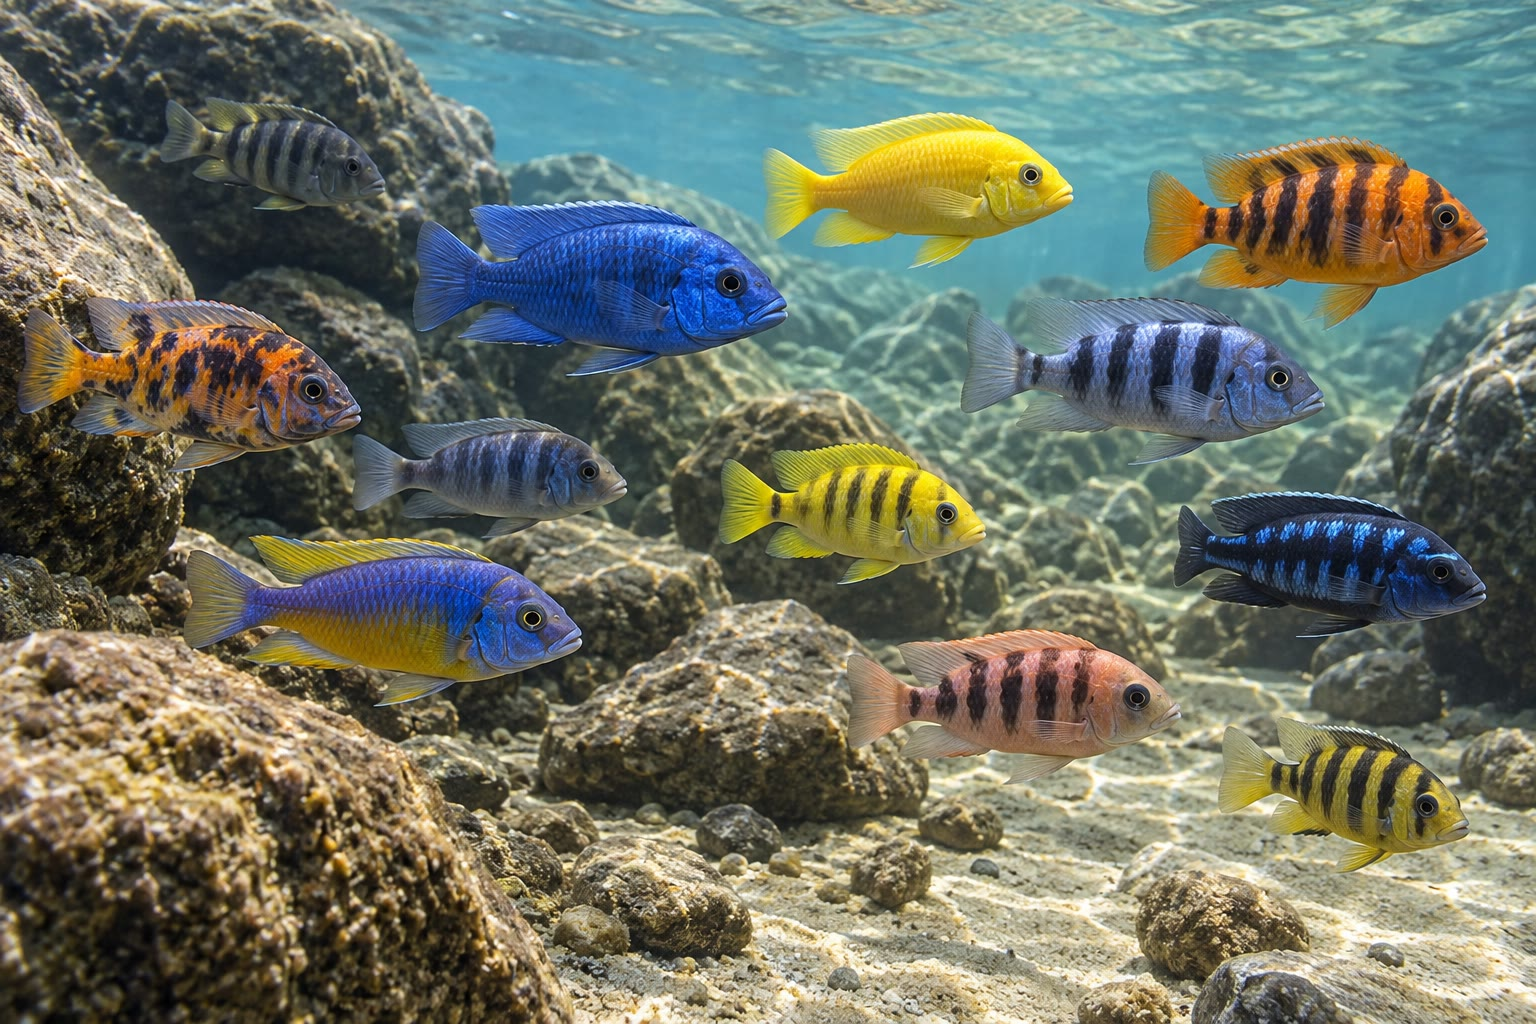
\includegraphics[width=0.6\linewidth]{images/book5/ai/b5-25-cichlids.jpg}

{\small Des cichlidés d'un lac africain~: des centaines d'espèces en
quelques milliers d'années, leurs différences tirées pour l'essentiel de
la variation que leurs ancêtres communs portaient déjà.}
\end{omfigure}

\begin{remark}[Le hasard comme référence]\label{rem:b3:molecular-evolution:remark}
La \omterm{thm:b3:molecular-evolution:neutral}{théorie neutraliste} n'affirme pas que la sélection est sans
importance~; elle énonce ce qui arrive quand la sélection est absente,
assez précisément pour qu'on puisse l'éprouver. Parce que le taux neutre
est le taux de mutation, la divergence mesure le temps~; parce que le
changement neutre remplit les sites que la sélection laisse libres,
$\omega$ mesure la contrainte~; parce que les lignées neutres coalescent
à un taux connu, le désaccord des \omterm{prop:b3:molecular-evolution:ils}{arbres de gènes} mesure la taille de
populations que personne n'a vues. La sélection est alors ce qui reste
quand on a soustrait le hasard --- un gène dont l'$\omega$ dépasse un,
un balayage qui a vidé une région de sa variation, un arbre qui diverge
dans un sens que la dérive ne peut expliquer. L'antigel du poisson des
glaces de l'Antarctique, le lysozyme stomacal du ruminant, la troisième
opsine du primate sont les exceptions trouvées ainsi, et chacune est
l'histoire d'un gène copié et d'un nouveau travail. Le reste du génome
est une horloge.
\end{remark}

\section{Exercices}

\begin{exercise}[$\star$]\label{exo:b3:molecular-evolution:1}
Énoncer le \omterm{thm:b3:molecular-evolution:neutral}{taux de substitution} neutre et expliquer avec des mots
pourquoi il ne dépend pas de la taille de la population.
\end{exercise}

\begin{exercise}[$\star$]\label{exo:b3:molecular-evolution:2}
Définir \omterm{def:b3:genomics:comparative}{orthologue}, \omterm{def:b3:genomics:comparative}{paralogue} et \omterm{def:b3:molecular-evolution:duplication}{pseudogène}, avec un exemple de chacun
tiré de la famille des globines.
\end{exercise}

\begin{exercise}[$\star$]\label{exo:b3:molecular-evolution:3}
Que mesure $\omega = d_{N}/d_{S}$~? Interpréter $\omega = 0.02$,
$\omega = 1.0$ et $\omega = 2.5$, et nommer un gène de chaque sorte.
\end{exercise}

\begin{exercise}[$\star$]\label{exo:b3:molecular-evolution:4}
Pourquoi Kimura a-t-il conclu que la plupart des substitutions sont
neutres~? Redire l'argument avec les nombres de l'ouverture du chapitre.
\end{exercise}

\begin{exercise}[$\star\star$]\label{exo:b3:molecular-evolution:5}
$N = 5000$. Calculer la \omterm{thm:b3:molecular-evolution:neutral}{probabilité de fixation} d'une nouvelle mutation
avec $s
= 0$, $s = 0.001$, $s = 0.01$ et $s = -0.001$, à l'aide de la formule de
Kimura, et commenter lesquelles sont effectivement neutres.
\end{exercise}

\begin{exercise}[$\star\star$]\label{exo:b3:molecular-evolution:6}
Deux espèces diffèrent en \qty{12}{\%} des sites d'un gène dont le taux
neutre vaut \qty{2e-9}{} par site et par an. Estimer leur temps de
divergence avec et sans la correction de Jukes--Cantor. Pour quelle
différence brute la correction atteint-elle un facteur deux~?
\end{exercise}

\begin{exercise}[$\star\star$]\label{exo:b3:molecular-evolution:7}
Un gène de 300 codons a 700 sites non synonymes et 200 sites synonymes.
Entre deux espèces il montre 7 différences non synonymes et 10
synonymes. Calculer $p_{N}$, $p_{S}$ et $\omega$ (non corrigés). Quel
régime de sélection~? Et si les comptes étaient 35 et 10~?
\end{exercise}

\begin{exercise}[$\star\star$]\label{exo:b3:molecular-evolution:8}
Les séquences neutres de l'humain et du chimpanzé diffèrent en
\qty{1.2}{\%}~; la séparation date de \qty{6.5}{Myr}, le temps de
génération vaut \qty{25}{yr}. Estimer le taux de mutation par site et
par génération, et le nombre de mutations nouvelles dans un génome
diploïde de $6\times 10^{9}$ bases à chaque génération.
\end{exercise}

\begin{exercise}[$\star\star$]\label{exo:b3:molecular-evolution:9}
Avec $N = \num{50000}$ et $T = \num{100000}$ générations entre les deux
séparations, calculer la fraction d'\omterm{prop:b3:molecular-evolution:ils}{arbres de gènes} discordants avec
l'arbre des espèces pour l'humain, le chimpanzé et le gorille. Quel $T$
la porterait à \qty{10}{\%}~?
\end{exercise}

\begin{exercise}[$\star\star\star$]\label{exo:b3:molecular-evolution:10}
Montrer que la formule de Kimura se réduit à $1/2N$ quand $s \to 0$ et à
$2s$ pour $4Ns \gg 1$, et que pour $s < 0$ avec $4N|s| \gg 1$ elle se
comporte comme $2|s|\,\mathrm{e}^{-4N|s|}$. En déduire à quel point une
mutation doit être délétère, dans une population de $10^{4}$, pour que
sa \omterm{thm:b3:molecular-evolution:neutral}{probabilité de fixation} soit cent fois plus faible que celle d'une
mutation neutre.
\end{exercise}

\begin{exercise}[$\star\star\star$]\label{exo:b3:molecular-evolution:11}
Un test de taux relatifs~: un groupe externe $O$ est à la distance
corrigée $0.30$ de la souris et $0.24$ de l'humain, et la souris et
l'humain sont à $0.20$ l'un de l'autre. Calculer les longueurs de
branche de la souris et de l'humain depuis leur séparation (en supposant
le point de séparation équidistant d'$O$ sur les deux chemins), et leur
rapport. Avec une génération de souris de \qty{0.5}{yr} et une
génération humaine de \qty{25}{yr}, que prédirait une horloge stricte
par génération pour ce rapport, et que dit l'observation des taux de
mutation par génération~?
\end{exercise}

\begin{exercise}[$\star\star\star$]\label{exo:b3:molecular-evolution:12}
Un gène dupliqué est libéré de toute contrainte ($\omega = 1$) au taux
neutre $k = \qty{2e-9}{}$ par site et par an. Dans une séquence codante
de 1000 bases, au bout de combien d'années environ attend-on le premier
codon stop ou décalage du cadre (supposer qu'environ \qty{4}{\%} des
mutations ponctuelles au hasard dans une séquence codante créent un
codon stop, et négliger les indels)~? Comparer au temps dont dispose la
sélection pour trouver une fonction nouvelle, et expliquer pourquoi la
plupart des duplicats meurent.
\end{exercise}

\section{Problème~: le rythme du changement}

\begin{problem}[{Problème du week-end --- l'histoire d'un génome en
chiffres~: le taux de mutation tiré de la divergence humain--chimpanzé,
la charge de substitution de Kimura, les chances de fixation des
mutations sélectionnées, l'$\omega$ d'un gène tiré de comptes de codons,
l'horloge lue pour une duplication, et la discordance des arbres de
gènes chez les grands singes, pour finir sur le taux de mutation,
l'$\omega$ du gène et la fraction discordante}]
\label{pb:b3:molecular-evolution:1}
Données~: divergence neutre humain--chimpanzé $d = 0.012$~; séparation
il y a \qty{6.5}{Myr}~; génération \qty{25}{yr}~; génome diploïde de
$6\times
10^{9}$ bases, \qty{1.5}{\%} de codant. Population ancestrale $N =
\num{50000}$. Gène~: 400 codons, 920 sites non synonymes et 280 sites
synonymes~; différences humain--souris 46 non synonymes et 84 synonymes.
Séparation humain--souris \qty{90}{Myr}. Globine~: $\alpha$ et $\beta$
diffèrent en \qty{55}{\%} des sites d'acides aminés (brut)~; taux de
l'hémoglobine \num{1e-9} par site et par an. Grands singes~: $T$ entre
les séparations du gorille et du chimpanzé \num{80000} générations.
Limite de Haldane~: une substitution sélectionnée par 300 générations.

\medskip
\noindent\textbf{Partie I --- Le taux.}
\begin{enumerate}
  \item À partir de $d = 2kT$, calculer $k$ par site et par an, puis
        $\mu$ par site et par génération.
  \item Mutations nouvelles par génome diploïde et par génération, et
        combien d'entre elles tombent dans du codant.
  \item Substitutions fixées par génération dans tout le génome au taux
        neutre (la population fixe $\mu$ par site et par génération).
        Comparer à la limite de Haldane et tirer la conclusion de Kimura.
  \item Dans une population de $N = \num{50000}$, combien de mutations
        neutres nouvelles apparaissent par site et par génération dans
        toute la population, et quelle fraction d'entre elles se fixera
        un jour~?
  \item Combien de temps met une mutation neutre destinée à se fixer, en
        générations et en années~? Comparer au temps écoulé depuis la
        séparation humain--chimpanzé.
  \item Expliquer pourquoi, malgré la question~5, la divergence entre
        deux espèces mesure le temps écoulé depuis leur séparation et non
        celui écoulé depuis la fixation de leurs allèles.
\end{enumerate}

\medskip
\noindent\textbf{Partie II --- Les chances de la sélection.}
\begin{enumerate}[resume]
  \item \omterm{thm:b3:molecular-evolution:neutral}{Probabilité de fixation} d'une mutation neutre dans
        $N = \num{50000}$, et d'une mutation à $s = 0.001$, $s = 0.01$,
        $s = 0.1$.
  \item Pour quel $s$ a-t-on $4Ns = 1$~? Interpréter la frontière.
  \item Une mutation délétère à $s = -0.001$~: \omterm{thm:b3:molecular-evolution:neutral}{probabilité de fixation}
        rapportée à la neutre. Et à $s = -10^{-5}$~?
  \item Si une fraction $10^{-5}$ des mutations nouvelles d'un gène sont
        bénéfiques avec $s = 0.01$ et le reste neutre, quelle fraction
        des substitutions de ce gène est adaptative~? Commenter la
        rareté avec laquelle la sélection se voit dans la séquence, même
        quand elle agit.
  \item Calculer $p_{N}$ et $p_{S}$ pour le gène humain--souris, corriger
        chacun par Jukes--Cantor, et donner $\omega$.
  \item Interpréter $\omega$~; et estimer le taux neutre qu'implique le
        $d_{S}$ du gène (par site et par an) à l'aide du temps de
        séparation. Est-ce cohérent avec la question~1~?
\end{enumerate}

\medskip
\noindent\textbf{Partie III --- Horloges et copies.}
\begin{enumerate}[resume]
  \item Corriger la différence entre les globines $\alpha$ et $\beta$
        pour les coups multiples (employer $d = -\ln(1 - p)$, la version
        protéique à nombreux états), et dater la duplication avec le taux
        de l'hémoglobine.
  \item La date tombe près de l'origine des vertébrés à mâchoires
        (\qtyrange{450}{500}{Myr}). Qu'autorisent des chaînes $\alpha$ et
        $\beta$ séparées qu'une chaîne unique n'autorise pas~?
  \item Les fibrinopeptides changent à $8\times 10^{-9}$ par site et par
        an. Deux espèces séparées depuis \qty{40}{Myr}~: différence brute
        attendue~? Pourquoi cette protéine est-elle inutile pour dater
        des séparations de \qty{500}{Myr}~?
  \item L'\omterm{def:b3:chromatin-epigenetics:nucleosome}{histone} H4 change à $10^{-11}$~: combien de substitutions sur
        100 sites en \qty{1000}{Myr}~? Pourquoi est-elle inutile pour
        dater des séparations récentes~?
  \item Un gène dupliqué dérive avec $\omega = 1$ dès la duplication. Si
        \qty{4}{\%} des substitutions dans du codant créent un stop, et
        que le gène a 1200 sites au taux $2\times
        10^{-9}$ par site et par an, estimer le temps attendu jusqu'au
        premier codon stop.
  \item Pourquoi une \omterm{def:b3:genomics:comparative}{duplication du génome entier} donne-t-elle aux
        duplicats une meilleure chance de survie qu'une simple
        duplication en tandem~?
\end{enumerate}

\medskip
\noindent\textbf{Partie IV --- Des arbres dans des arbres.}
\begin{enumerate}[resume]
  \item Probabilité qu'une lignée humaine et une lignée de chimpanzé ne
        coalescent pas dans les \num{80000} générations qui précèdent la
        séparation du gorille.
  \item Fraction d'\omterm{prop:b3:molecular-evolution:ils}{arbres de gènes} discordants avec l'arbre des espèces.
        Observé~: environ \qty{30}{\%}. Est-ce cohérent~?
  \item Parmi les arbres discordants, quelle fraction groupe l'humain
        avec le gorille, et quelle fraction le chimpanzé avec le
        gorille~? Qu'indiquerait un écart marqué à l'égalité~?
  \item Si la population ancestrale avait valu $N = \num{10000}$, quelle
        fraction discordante attendre~? Que dit donc la fraction
        observée des effectifs de nos ancêtres~?
  \item Pourquoi concaténer mille gènes en un seul \omterm{def:b3:bioinformatics:alignment}{alignement} donne-t-il
        un arbre assuré mais possiblement faux, et que fait à la place
        une méthode fondée sur le coalescent~?
  \item L'ADN de Néandertal chez les humains non africains fait environ
        \qty{2}{\%} et les arbres qui le portent groupent certains
        Européens avec les Néandertaliens plus souvent que les
        Africains. Pourquoi n'est-ce pas un \omterm{prop:b3:molecular-evolution:ils}{tri incomplet des lignées}~?
  \item Résumer~: $\mu$ (question~1), l'$\omega$ du gène (question~11),
        et la fraction discordante (question~20).
\end{enumerate}
\end{problem}
